\section{Existing simulators}
\label{sec:existing}

\subsection{simglucose}
\label{sec:simglucose}

\begin{figure}
    \centering
    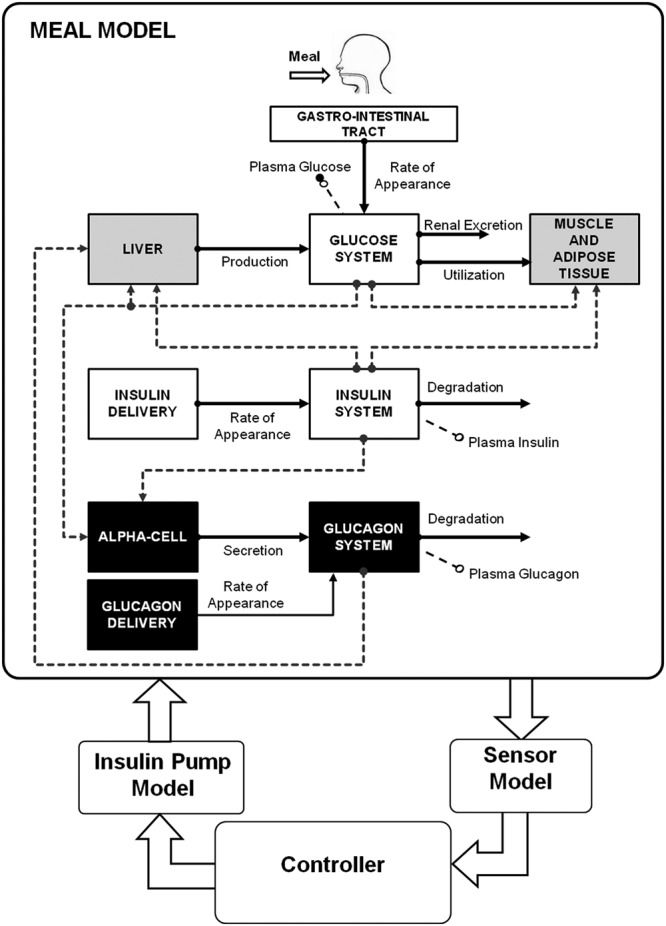
\includegraphics[width=\linewidth]{uvapadova.jpg}
    \caption{UVA/PADOVA equations, visualised}
    \label{fig:uvapadova}
\end{figure}

UVA/Padova \cite{sim-diabetes-fda} is a set of equations used to model type 1 diabetes.
The equations, outlined on figure \ref{fig:uvapadova}, were developed by clinical experts and validated on a dataset of 32 people aged 38 ± 12 years.
It is widely used in Healthcare and even approved in the United States as a replacement for clinical trials.
It provides $\prob_\obs(\obs | \state, \action)$ and $\prob_s(\state_\text{next} | \state_\text{prev}, \action)$ (see section \ref{sec:rlcef}), so to be a full-fledged Markov Decision Process it only needs $\prob_r(r|\state,\action)$.
\cite{simglucose} solves exactly that by adding a reward function based on diabetes risk index as defined in \cite{diabetesrisk} to the UVA/Padova simulator, providing a Reinforcement Learning environment for type 1 diabetes.

\subsection{GYMIC}
\label{sec:gymic}

\subsubsection{Scope}
GYMIC \cite{gym-sepsis} is, unlike the previous examples, a fully data-driven simulator. 
It harnesses a subset of MIMIC \cite{johnsonMIMICIVFreelyAccessible2023} dataset to address on one of the most challenging problems in emergency care - sepsis.
The authors intentionally limit their scope to just sepsis in order to simplify the modelling task as well as because sepsis prevention has been identified as an area where doctors would particularly benefit from electronic decision support \cite{sepsis-motivation1,sepsis-motivation2}.

\subsubsection{Prediction model}
The prediction model of GYMIC simulator is defined as a solution to the following autoregression task:
\begin{enumerate}
    \item A clinical history is a sequence of $(\state, \action)$ tuples
    \item $\action \in 0,\dots 24$ is one of 25 possible vasopressor or intravenous fluid interventions - a cartensian product of 5 types of interventions and 5 dosage quantiles. 
    \item $\state \in R^{46}$ is the patient's state at the moment this intervention was administered.
    \item Predict the conditional state distribution $\prob_s(\state_\step, \action_\step | \state_{\step-1},\state_{\step-2},\dots,\state_1)$
\end{enumerate}

The dataset of clinical histories is produced by \action preprocessing algorithm combining together all clinical records from MIMIC that relate to sepsis patients.

Autoregressive tasks of this nature arise in many fields like stock market prediction \cite{stonks1,stonks2} or language modelling \cite{langmodels} where state of the art solutions can be found.
The authors of \emph{GYMIC} solve it with an LSTM \cite{hochreiterLongShorttermMemory1997} neural network with 2 additional dense layers attached, see figure \ref{fig:gymic} for the diagram.
Faced with some of the mode collapse issues described in section \ref{sec:gymic-results} the authors also experimented with semi-supervised learning \cite{semi-supervised}: they trained \action variational autoencoder \cite{vae} on all patient states to replace the 46-vector representations of patient state $\state$ with learned representations from the latent space of the VAE $\text{encoder}(\state)$.
The issues persisted.

\begin{figure}
    \centering
    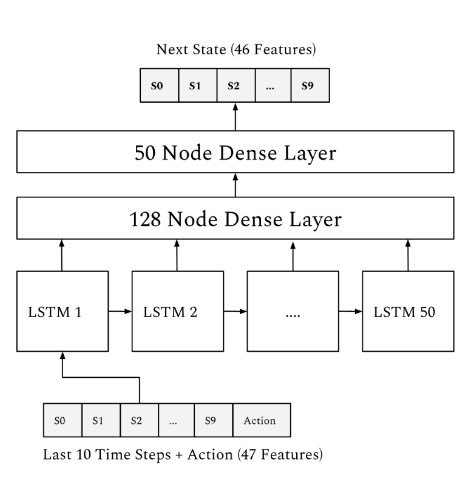
\includegraphics[width=\linewidth]{gymic.png}
    \caption{Neural architecture of GYMIC}
    \label{fig:gymic}
\end{figure}

\subsubsection{Reward model}

Highlighting the gravity of contracting sepsis, \emph{GYMIC} has only 2 outcomes: patient is discharged from intensive care or patient dies.
Its reward model reflects that, giving the agent a large positive or negative reward at the end of the episode, depending on the outcome.
However, in order to lower the difficulty of the simulator (delayed gratification makes training significantly harder \cite{delayedgrat-humans, delayedgrat-ai}) an additional reward is provided during the episode, based on the evolution of the patient's SOFA score \cite{sofa} - a commonly used measure of sepsis severity:

\begin{multline}
r\left(\state_{\step}, \state_{\step+1}\right)=C_{0} \mathbb{1}\left(\state_{\step+1}^{\mathrm{SOFA}}=\state_{\step}^{\mathrm{SOFA}} \& \state_{\step+1}^{\text {SOFA }}>0\right) + \\ +
C_{1}\left(\state_{\step+1}^{\mathrm{SOFA}}-\state_{\step}^{\mathrm{SOFA}}\right) + 
C_{2} \tanh \left(\state_{\step+1}^{\text {Lactate }}-\state_{\step}^{\text {Lactate }}\right)
\end{multline}

A third reward component is proposed to negatively reinforce action severity and encourage the agent to use low doses of drugs - an instance of \emph{confirmation bias} as discussed in section \ref{sec:bias}, but a necessary step given the issues in section \ref{sec:gymic-results}.

\subsubsection{Results and issues}
\label{sec:gymic-results}

Unfortunately, the experiments performed by the authors of \emph{GYMIC} indicate extreme overfitting.
Due to \emph{sampling bias} and simply inadequate size of the dataset there are treatments that have only occurred a few times in the training data and have always resulted in a positive health outcome.
In \emph{GYMIC} these treatments are silver bullets that guarantee a successful outcome while in real life they are risky and potentially very harmful.
